%\documentclass{beamer} 
\documentclass[handout]{beamer} % sin pausas
\usetheme{CambridgeUS}
%\setbeamertemplate{background}[grid][step=8 ] % cuadriculado

\usepackage{etex}
\usepackage{t1enc}
\usepackage[spanish,es-nodecimaldot]{babel}
\usepackage{latexsym}
\usepackage[utf8]{inputenc}
\usepackage{verbatim}
\usepackage{multicol}
\usepackage{amsgen,amsmath,amstext,amsbsy,amsopn,amsfonts,amssymb}
\usepackage{amsthm}
\usepackage{calc}         % From LaTeX distribution
\usepackage{graphicx}     % From LaTeX distribution
\usepackage{ifthen}
%\usepackage{makeidx}
\input{random.tex}        % From CTAN/macros/generic
\usepackage{subfigure} 
\usepackage{tikz}
\usepackage[customcolors]{hf-tikz}
\usepackage[most]{tcolorbox}
\usetikzlibrary{arrows}
\usetikzlibrary{matrix}
\tikzset{
    every picture/.append style={
        execute at begin picture={\deactivatequoting},
        execute at end picture={\activatequoting}
    }
}
\usetikzlibrary{decorations.pathreplacing,angles,quotes}
\usetikzlibrary{shapes.geometric}
\usepackage{mathtools}
\usepackage{stackrel}
%\usepackage{enumerate}
\usepackage{enumitem}
\usepackage{tkz-graph}
\usepackage{polynom}
\polyset{%
    style=B,
    delims={(}{)},
    div=:
}
\renewcommand\labelitemi{$\circ$}
\setlist[enumerate]{label={(\arabic*)}}
%\setbeamertemplate{background}[grid][step=8 ] % cuadriculado
\setbeamertemplate{itemize item}{$\circ$}
\setbeamertemplate{enumerate items}[default]
\definecolor{links}{HTML}{2A1B81}
\hypersetup{colorlinks,linkcolor=,urlcolor=links}


\newcommand{\Id}{\operatorname{Id}}
\newcommand{\img}{\operatorname{Im}}
\newcommand{\nuc}{\operatorname{Nu}}
\newcommand{\im}{\operatorname{Im}}
\renewcommand\nu{\operatorname{Nu}}
\newcommand{\la}{\langle}
\newcommand{\ra}{\rangle}
\renewcommand{\t}{{\operatorname{t}}}
\renewcommand{\sin}{{\,\operatorname{sen}}}
\newcommand{\Q}{\mathbb Q}
\newcommand{\R}{\mathbb R}
\newcommand{\C}{\mathbb C}
\newcommand{\K}{\mathbb K}
\newcommand{\F}{\mathbb F}
\newcommand{\Z}{\mathbb Z}
\newcommand{\N}{\mathbb N}
\newcommand\sgn{\operatorname{sgn}}
\renewcommand{\t}{{\operatorname{t}}}
\renewcommand{\figurename }{Figura}

%
% Ver http://joshua.smcvt.edu/latex2e/_005cnewenvironment-_0026-_005crenewenvironment.html
%

\renewenvironment{block}[1]% environment name
{% begin code
	\par\vskip .2cm%
	{\color{blue}#1}%
	\vskip .2cm
}%
{%
	\vskip .2cm}% end code


\renewenvironment{alertblock}[1]% environment name
{% begin code
	\par\vskip .2cm%
	{\color{red!80!black}#1}%
	\vskip .2cm
}%
{%
	\vskip .2cm}% end code


\renewenvironment{exampleblock}[1]% environment name
{% begin code
	\par\vskip .2cm%
	{\color{blue}#1}%
	\vskip .2cm
}%
{%
	\vskip .2cm}% end code




\newenvironment{exercise}[1]% environment name
{% begin code
	\par\vspace{\baselineskip}\noindent
	\textbf{Ejercicio (#1)}\begin{itshape}%
		\par\vspace{\baselineskip}\noindent\ignorespaces
	}%
	{% end code
	\end{itshape}\ignorespacesafterend
}


\newenvironment{definicion}[1][]% environment name
{% begin code
	\par\vskip .2cm%
	{\color{blue}Definición #1}%
	\vskip .2cm
}%
{%
	\vskip .2cm}% end code

    \newenvironment{notacion}[1][]% environment name
    {% begin code
        \par\vskip .2cm%
        {\color{blue}Notación #1}%
        \vskip .2cm
    }%
    {%
        \vskip .2cm}% end code

\newenvironment{observacion}[1][]% environment name
{% begin code
	\par\vskip .2cm%
	{\color{blue}Observación #1}%
	\vskip .2cm
}%
{%
	\vskip .2cm}% end code

\newenvironment{ejemplo}[1][]% environment name
{% begin code
	\par\vskip .2cm%
	{\color{blue}Ejemplo #1}%
	\vskip .2cm
}%
{%
	\vskip .2cm}% end code


\newenvironment{preguntas}[1][]% environment name
{% begin code
    \par\vskip .2cm%
    {\color{blue}Preguntas #1}%
    \vskip .2cm
}%
{%
    \vskip .2cm}% end code

\newenvironment{ejercicio}[1][]% environment name
{% begin code
	\par\vskip .2cm%
	{\color{blue}Ejercicio #1}%
	\vskip .2cm
}%
{%
	\vskip .2cm}% end code


\renewenvironment{proof}% environment name
{% begin code
	\par\vskip .2cm%
	{\color{blue}Demostración}%
	\vskip .2cm
}%
{%
	\vskip .2cm}% end code



\newenvironment{demostracion}% environment name
{% begin code
	\par\vskip .2cm%
	{\color{blue}Demostración}%
	\vskip .2cm
}%
{%
	\vskip .2cm}% end code

\newenvironment{idea}% environment name
{% begin code
	\par\vskip .2cm%
	{\color{blue}Idea de la demostración}%
	\vskip .2cm
}%
{%
	\vskip .2cm}% end code

\newenvironment{solucion}% environment name
{% begin code
	\par\vskip .2cm%
	{\color{blue}Solución}%
	\vskip .2cm
}%
{%
	\vskip .2cm}% end code



\newenvironment{lema}[1][]% environment name
{% begin code
	\par\vskip .2cm%
	{\color{blue}Lema #1}\begin{itshape}%
		\par\vskip .2cm
	}%
	{% end code
	\end{itshape}\vskip .2cm\ignorespacesafterend
}

\newenvironment{proposicion}[1][]% environment name
{% begin code
	\par\vskip .2cm%
	{\color{blue}Proposición #1}\begin{itshape}%
		\par\vskip .2cm
	}%
	{% end code
	\end{itshape}\vskip .2cm\ignorespacesafterend
}

\newenvironment{teorema}[1][]% environment name
{% begin code
	\par\vskip .2cm%
	{\color{blue}Teorema #1}\begin{itshape}%
		\par\vskip .2cm
	}%
	{% end code
	\end{itshape}\vskip .2cm\ignorespacesafterend
}


\newenvironment{corolario}[1][]% environment name
{% begin code
	\par\vskip .2cm%
	{\color{blue}Corolario #1}\begin{itshape}%
		\par\vskip .2cm
	}%
	{% end code
	\end{itshape}\vskip .2cm\ignorespacesafterend
}

\newenvironment{propiedad}% environment name
{% begin code
	\par\vskip .2cm%
	{\color{blue}Propiedad}\begin{itshape}%
		\par\vskip .2cm
	}%
	{% end code
	\end{itshape}\vskip .2cm\ignorespacesafterend
}

\newenvironment{conclusion}% environment name
{% begin code
	\par\vskip .2cm%
	{\color{blue}Conclusión}\begin{itshape}%
		\par\vskip .2cm
	}%
	{% end code
	\end{itshape}\vskip .2cm\ignorespacesafterend
}


\newenvironment{definicion*}% environment name
{% begin code
	\par\vskip .2cm%
	{\color{blue}Definición}%
	\vskip .2cm
}%
{%
	\vskip .2cm}% end code

\newenvironment{observacion*}% environment name
{% begin code
	\par\vskip .2cm%
	{\color{blue}Observación}%
	\vskip .2cm
}%
{%
	\vskip .2cm}% end code


\newenvironment{obs*}% environment name
	{% begin code
		\par\vskip .2cm%
		{\color{blue}Observación}%
		\vskip .2cm
	}%
	{%
		\vskip .2cm}% end code

\newenvironment{ejemplo*}% environment name
{% begin code
	\par\vskip .2cm%
	{\color{blue}Ejemplo}%
	\vskip .2cm
}%
{%
	\vskip .2cm}% end code

\newenvironment{ejercicio*}% environment name
{% begin code
	\par\vskip .2cm%
	{\color{blue}Ejercicio}%
	\vskip .2cm
}%
{%
	\vskip .2cm}% end code

\newenvironment{propiedad*}% environment name
{% begin code
	\par\vskip .2cm%
	{\color{blue}Propiedad}\begin{itshape}%
		\par\vskip .2cm
	}%
	{% end code
	\end{itshape}\vskip .2cm\ignorespacesafterend
}

\newenvironment{conclusion*}% environment name
{% begin code
	\par\vskip .2cm%
	{\color{blue}Conclusión}\begin{itshape}%
		\par\vskip .2cm
	}%
	{% end code
	\end{itshape}\vskip .2cm\ignorespacesafterend
}






\newcommand{\nc}{\newcommand}

%%%%%%%%%%%%%%%%%%%%%%%%%LETRAS

\nc{\FF}{{\mathbb F}} \nc{\NN}{{\mathbb N}} \nc{\QQ}{{\mathbb Q}}
\nc{\PP}{{\mathbb P}} \nc{\DD}{{\mathbb D}} \nc{\Sn}{{\mathbb S}}
\nc{\uno}{\mathbb{1}} \nc{\BB}{{\mathbb B}} \nc{\An}{{\mathbb A}}

\nc{\ba}{\mathbf{a}} \nc{\bb}{\mathbf{b}} \nc{\bt}{\mathbf{t}}
\nc{\bB}{\mathbf{B}}

\nc{\cP}{\mathcal{P}} \nc{\cU}{\mathcal{U}} \nc{\cX}{\mathcal{X}}
\nc{\cE}{\mathcal{E}} \nc{\cS}{\mathcal{S}} \nc{\cA}{\mathcal{A}}
\nc{\cC}{\mathcal{C}} \nc{\cO}{\mathcal{O}} \nc{\cQ}{\mathcal{Q}}
\nc{\cB}{\mathcal{B}} \nc{\cJ}{\mathcal{J}} \nc{\cI}{\mathcal{I}}
\nc{\cM}{\mathcal{M}} \nc{\cK}{\mathcal{K}}

\nc{\fD}{\mathfrak{D}} \nc{\fI}{\mathfrak{I}} \nc{\fJ}{\mathfrak{J}}
\nc{\fS}{\mathfrak{S}} \nc{\gA}{\mathfrak{A}}
%%%%%%%%%%%%%%%%%%%%%%%%%LETRAS

\title[Clase 5 - Inducción]{Matemática Discreta I \\ Clase 5 - Inducción completa - Conteo}
%\author[C. Olmos / A. Tiraboschi]{Carlos Olmos / Alejandro Tiraboschi}
\institute[]{\normalsize FAMAF / UNC
    \\[\baselineskip] ${}^{}$
    \\[\baselineskip]
}
\date[30/03/2023]{30 de marzo   de 2023}




\begin{document}

\frame{\titlepage} 



\begin{frame}\frametitle{} 

    Practiquemos un poco con inducción.

    \begin{ejercicio}
        Probar que 
        $$
            1^3 +2^3 +3^3 + \cdots +n^3 = \frac{n^2(n+1)^2}{4},
        $$
        para $n \in \N$.
    \end{ejercicio}\pause
\begin{proof}\pause
    \vskip .4cm 
    \noindent({\it Caso  base})\pause El resultado es verdadero
        cuando $n=1$ pues 
        $$ \sum_{i=1}^{1} i^3 = 1\quad \text{y}\quad\frac{1^2(1+1)^2}{4} =\frac{4}{4} =1.$$
    
\end{proof}
\end{frame}


\begin{frame}
    \frametitle{}


        
        \vskip 1cm \pause
        \noindent ({\it Paso  inductivo})\pause
        Debemos probar que si $k \ge 1$, 
        \vskip 0.4cm 
        $$
        \sum_{i=1}^{k} i^3 = \frac{k^2(k+1)^2}{4} \;\; \text{ (HI) }\quad \Rightarrow \quad    \sum_{i=0}^{k+1} i^3 =\frac{(k+1)^2(k+2)^2}{4}.
        $$

    

\end{frame}


\begin{frame}
    \frametitle{}
    
    \begin{tabular}{lllll}
        $\displaystyle\sum_{i=1}^{k+1} i^3$ &$=$& $\displaystyle\sum_{i=1}^{k} i^3 + (k+1)^3$ &\qquad &$\text{(por la definición recursiva de $\sum$ )}$ \\[0.6cm]
    &$=$& $\displaystyle\frac{k^2(k+1)^2}{4}+(k+1)^3$ &\quad &$\text{(por hipótesis inductiva)}$ \\[0.6cm]
    &$=$& $\displaystyle(k+1)^2(\frac{k^2}{4}+(k+1)))$ &\quad &$\text{($(k+1)^2$ factor común)}$ \\[0.6cm]
    &$=$& $\displaystyle(k+1)^2\frac{(k^2+4k+4)}{4}.$&\quad &\\[0.6cm]
    &$=$& $\displaystyle\frac{(k+1)^2(k+2)^2}{4}.$&\quad &
    \end{tabular}
    \medskip
    \pause
    
    Luego el resultado es verdadero cuando $n=k+1$ y por el principio de inducción, es verdadero para todos los enteros positivos $n$.\qed

\end{frame}

\begin{frame}
    \frametitle{Inducción completa}
    Existen varias formas modificadas del principio de inducción. A veces es conveniente tomar como base inductiva el valor $n=0$, por otro lado puede ser apropiado tomar un valor como $2$ o $3$ porque los primeros casos pueden ser excepcionales. 
    \pause
    \medskip
    
    Cada problema debe ser tratado según sus características. 
    \pause
    \medskip
    
    Otra modificación útil es tomar como hipótesis inductiva la suposición de que el resultado es verdadero para todos los valores $n\le k$, más que para $n=k$ solamente.
    \pause
    \medskip
    
    Esta formulación es llamada a veces el {\it principio de inducción completa}. Todas esas modificaciones pueden justificarse con cambios triviales en la demostración del principio de inducción.
    
\end{frame}

\begin{frame}    
    El siguiente teorema incorpora muchas de las modificaciones del principio de inducción mencionadas más arriba.

    \pause
    \medskip
    

    
    %\begin{teorema}[Inducción completa]\label{ind-completa} 
    {\color{blue} Teorema (Inducción completa)}
    \vskip .2cm    
        Sea $n_0$ número entero y sea $P(n)$ una propiedad para $n \ge n_0$ tal que:
        \begin{enumerate}
            \item[a)] $P(n_0)$ es verdadera.
            \item[b)] Si $P(h)$ verdadera para toda $h$ tal que $n_0 \le h \le k$ implica $P(k + 1)$ verdadera.
        \end{enumerate}
        Entonces $P(n)$ es verdadera para todo $n \ge n_0$.
    %\end{teorema}

    
\end{frame}



\begin{frame}        
    
    \begin{ejemplo}
        $$u_1 = 3,\qquad u_2 = 5,\qquad u_n = 3u_{n-1}- 2u_{n-2},\qquad  n \ge 3.$$
        Probemos que $u_n = 2^n + 1$, para todo $n \in  \mathbb N$.
    \end{ejemplo}
        {\color{blue} Solución.}
        \vskip .2cm    
        \pause
            
            \noindent({\it Caso  base})
            
            \setbeamercolor{postit}{fg=black,bg=example text.fg!75!black!10!bg}
        \hskip 2.5cm\begin{beamercolorbox}[wd=0.65\textwidth,rounded=true,shadow=true]{postit}
            $n= \colorbox{blue!30}{1}$ :  $3 = 2^1+1$ \checkmark, \qquad   $n=\colorbox{green!50}{2}$ :  $ 5 =2^2+1$ \checkmark.
            \end{beamercolorbox} \pause
            
            \vskip.4cm
            
            \noindent ({\it Paso  inductivo}) Hipótesis inductiva:
            \vskip.2cm
            \setbeamercolor{postit}{fg=black,bg=example text.fg!75!black!10!bg}
            \hskip 2.5cm\begin{beamercolorbox}[wd=0.65\textwidth,rounded=true,shadow=true]{postit}
            \quad $u_h = 2^h+1$  para  $\colorbox{blue!30}{1} \le h \le k$   y  $k \ge \colorbox{green!50}{2}$  (HI),  
        \end{beamercolorbox}
            \pause
            \vskip.2cm
        Luego debemos probar que:
\end{frame}

\begin{frame}
    \frametitle{}
    \setbeamercolor{postit}{fg=black,bg=example text.fg!75!black!10!bg}
    \hskip 0.5cm\begin{beamercolorbox}[wd=0.9\textwidth,rounded=true,shadow=true]{postit}
        \quad $u_h = 2^h+1$  para  $1 \le h \le k$  (HI) \quad $\Rightarrow$ \quad
        $u_{k+1}=2^{k+1}+1.$  
    \end{beamercolorbox}    \pause
    \vskip.5cm
    Se  comienza con el término izquierdo de lo que se quiere probar y  se obtiene el derecho.     \pause
    \vskip.4cm
    \begin{tabular}{llll}
        $u_{k+1}$ &$= 3u_k -2u_{k-1}$ &\qquad &{(por definición recursiva)}  \\[0.2cm].
            &$= 3(2^k+1)-2(2^{k-1}+1)$  &\qquad &{(por hipótesis inductiva)} \\[0.2cm]
            &= $3\cdot 2^k+3-2\cdot 2^{k-1}-2$ &\qquad & \\[0.2cm]
            &= $3\cdot 2^k+1- 2^{k}$  &\qquad & \\[0.2cm]
            &= $2\cdot 2^k+1$  &\qquad & \\[0.2cm]
            &= $2^{k+1}+1.$  &\qquad & 
        \end{tabular}

\qed
\end{frame}



\begin{frame}
    

    \begin{ejercicio}
        Sea $u_n$ definida recursivamente por:
        \begin{equation*}
        u_0 = 1, \; u_1 = 0, \;\qquad u_n = 5u_{n-1} - 6 u_{n-2}, \; \forall n \ge 2. 
        \end{equation*}
        \begin{enumerate}
            \item[1.]  Calcule $u_2$ y $u_3$ usando  recursión.
            \item[2.] Pruebe por inducción que $u_n = 3\cdot 2^n - 2 \cdot 3^n$ ($n \in \N_0$). 
        \end{enumerate}
        \vskip .2cm
    \end{ejercicio}\pause

    \begin{solucion}\pause
        {\noindent 1.} Por definición $u_0 = 1, \; u_1 = 0$, luego:
        \begin{equation*}
        u_2 = 5u_{2-1} - 6 u_{2-2} = 5u_{1} - 6 u_{0} = 5 \cdot 0 - 6 \cdot 1 = -6 
        \end{equation*}\pause
        Ahora  $u_1 = 0, \; u_2 = -6$, luego:\pause
        \begin{equation*}
        u_3 = 5u_{3-1} - 6 u_{3-2} = 5u_{2} - 6 u_{1} = 5 \cdot (-6) - 6 \cdot 0 = -30. 
        \end{equation*}
    \end{solucion}

\end{frame}


\begin{frame}
    \frametitle{}


        {\noindent 2.} \noindent ({\it Caso base})\pause
        \vskip .2cm
        $n=\colorbox{blue!30}{0}$: por un lado $u_0 =1$, por definición, por otro lado  si calculamos con la fórmula: $u_0 = 3 \cdot 2^0 - 2 \cdot 3^0 = 3- 2 = 1$ y listo.
        \vskip .2cm\pause
        $n=\colorbox{green!50}{1}$: por un lado $u_1 =0$, por definición, por otro lado  si calculamos con la fórmula: $u_1 = 3 \cdot 2^1 - 2 \cdot 3^1 = 3 \cdot 2- 2 \cdot 3 =  6-6 = 0$ y listo.\pause
        
        \vskip .6cm
        
        \noindent ({\it Paso  inductivo}) \pause
        \vskip .2cm
        Debemos probar que si
        \begin{equation*}
            k \ge \colorbox{green!50}{1} \text{\; y\; } u_h = 3\cdot 2^h - 2 \cdot 3^h \text{ \;para\; }  \colorbox{blue!30}{0} \le h \le k, \tag{HI}
        \end{equation*}\pause
        eso implica que
        \begin{equation*}
        u_{k+1} = 3\cdot 2^{k+1} - 2 \cdot 3^{k+1}. \tag{*}
        \end{equation*}
        
\end{frame}


\begin{frame}
    \frametitle{}
    Comenzamos por el lado izquierdo de (*):
        \begin{align*}
        u_{k+1} &=   5u_{k+1-1} - 6 u_{k+1-2}&&\text{ \;(def. $u_n$)\; } \\
        &=   5u_{k} - 6 u_{k-1}&&\\
        &=   5( 3\cdot 2^{k} - 2 \cdot 3^{k}) - 6 ( 3\cdot 2^{k-1} - 2 \cdot 3^{k-1})&&\text{ \;(por HI)\; }
        \end{align*}\vskip .2cm
        En  lo que se refiere al procedimiento de inducción hemos terminado,  ahora solo queda por probar que
        \begin{equation}
            5( 3\cdot 2^{k} - 2 \cdot 3^{k}) - 6 ( 3\cdot 2^{k-1} - 2 \cdot 3^{k-1}) =
        3\cdot 2^{k+1} - 2 \cdot 3^{k+1} \tag{**}
        \end{equation}
        
        \vskip .2cm
        Desarrollemos el término de la izquierda
        \pause
        \begin{align*}
        \qquad &=  5( 3\cdot 2^{k} - 2 \cdot 3^{k}) - 6 ( 3\cdot 2^{k-1} - 2 \cdot 3^{k-1})&& \\
        &=   5\cdot  3\cdot 2^{k} - 5 \cdot 2 \cdot 3^{k} - 6 \cdot  3\cdot 2^{k-1} + 6 \cdot  2 \cdot 3^{k-1}&& \\
        &=   5\cdot  3\cdot 2^{k} - 5 \cdot 2 \cdot 3^{k} - 3 \cdot  3\cdot 2^{k} + 2 \cdot  2 \cdot 3^{k}&& \\
        &=   6\cdot 2^{k} - 6 \cdot 3^{k} && \\
        \end{align*}
        \pause
        
\end{frame}

\begin{frame}
    \frametitle{}
Luego (**) se transforma  en 
\begin{gather*}
    6\cdot 2^{k} - 6 \cdot 3^{k} =
    3\cdot 2^{k+1} - 2 \cdot 3^{k+1} \tag{***} \\
\Updownarrow\\
3\cdot 2 \cdot 2^{k} - 2 \cdot 3 \cdot 3^{k} =
    3\cdot 2^{k+1} - 2 \cdot 3^{k+1} \\
    \Updownarrow\\
    3\cdot 2^{k+1} - 2 \cdot 3^{k+1}  = 3\cdot 2^{k+1} - 2 \cdot 3^{k+1}. 
\end{gather*}

Como esto último es verdadero,  es verdadero (***) y por lo tanto son verdaderos (**) y (*). 

\qed

\end{frame}




\begin{frame}
    \frametitle{}

Nos adelantamos un poco en los temas de la materia para ejemplificar el principio de inducción completa aplicado a un problema que no es de recursión. 
\vskip .4cm\pause

\begin{definicion} Sea $n \in \N$ diremos que es \textit{primo} si $n \ne 1$ y el  único natural menor que lo divide es  $1$.
\end{definicion}
    \vskip .4cm\pause
\begin{ejercicio}
    Probar que si $n \in \N$, $n >1$,  entonces $n$  es producto de primos. 
\end{ejercicio}\pause

\begin{proof}\pause
    Lo haremos por inducción en $n \ge 2$. 
\end{proof}



\end{frame}


\begin{frame}
    \frametitle{}
    \noindent ({\it Caso base})\pause
    \vskip .4cm
    El caso base es $n=2$,  y es claro que $2$ es primo (y por lo tanto producto de primos  en un sentido generalizado).  
    \vskip .6cm\pause
    \noindent ({\it Paso inductivo})\pause
    \vskip .4cm
    Probaremos que dado $k\ge 2$, 

    \begin{gather*}
        \text{todo $h$ tal que $2 \le h \le k$, es producto de primos (HI)} \\[.2cm]
        \Downarrow \\[.2cm]
        \text{$k+1$  es producto de primos. }
    \end{gather*}

\end{frame}


\begin{frame}
    \frametitle{}
Si $k+1$ es primo, listo,  es producto de primos.\pause
\vskip .4cm
Si $k+1$ no es primo,  significa que $k+1= d \cdot e$ donde $d, e < k+1$. \pause
\vskip .4cm

Por (HI), $d$ y $e$ son productos de primos,  es decir
\begin{align*}
    d &= p_1\cdot p_2 \cdots p_r \\ 
    e &= q_1\cdot q_2 \cdots q_s \\ 
\end{align*}\vskip -.6cm
donde $p_i, q_i$ son primos.\pause Luego
\begin{equation*}
    k +1 = d \cdot e = p_1\cdot p_2 \cdots p_r \cdot q_1\cdot q_2 \cdots q_s. 
\end{equation*}
\vskip .4cm
\pause
Por lo tanto $k+1$  es producto de primos.

\qed
    

\end{frame}



\begin{frame}\frametitle{Problemas de conteo}     

    Contar,  a veces, no es una tarea sencilla. \pause

    \vskip .4cm

    Por ejemplo: \pause


    \begin{itemize}
        \item ¿Cuántas chapas patente  es posible hacer con el actual esquema de numeración? Nos referimos a las patentes de automóviles en Argentina.  \pause
        \item ¿De cuántas formas se pueden elegir 7 personas entre 20? (no importa el orden de la elección)
    \end{itemize}
    \pause
    \vskip .4cm

    En las próximas clases podremos resolver estos dos problemas utilizando \textit{técnicas de conteo.}
    \pause
    \vskip .4cm

    Las técnicas de conteo son estrategias matemáticas que permiten determinar el número total de resultados que pueden haber a partir de hacer combinaciones dentro de un conjunto o conjuntos de objetos.

\end{frame}

\begin{frame}\frametitle{Cardinal de un conjunto }     

    Un conjunto $A$ es finito si podemos contar la cantidad de elementos que tiene. En ese caso denotaremos $|A|$ la cantidad de elementos de $A$ y la llamaremos el {\em cardinal de $A$}. 
    
    A veces se denota también $\sharp A$.
    \pause
    \vskip .6cm
    Por  ejemplo, los conjuntos
    \begin{equation*}
        A = \{ a, b, z, x, 1\}, \qquad B = \{ 1, 2, 3, 4, 5\}
    \end{equation*}
    tienen 5 elementos cada uno. Es decir $|A| =5$ y $|B|= 5$.

    \vskip .6cm\pause

    Conjuntos como $\mathbb Z$, $\mathbb N$ o $\mathbb R$ son infinitos y por lo tanto no tiene sentido hablar de la cantidad de elementos de estos conjuntos.
\end{frame}

\begin{frame}\frametitle{El principio de adición}        
    Dadas dos actividades $X$ e $Y$, si se puede realizar $X$ de $n$ formas distintas o, alternativamente, se puede realizar  $Y$ de $m$ formas distintas. Entonces el número de formas de realizar ``$X$ o $Y$'' es $n + m$.

    \pause
    \vskip .4cm
    {\color{blue} Ejemplo}
    \vskip .2cm 
    Supongamos que una persona va a salir a pasear  y puede ir al cine donde hay $3$ películas en cartel o al teatro donde hay $4$ obras posibles. Entonces, tendrá un total de $3+4=7$ formas distintas de elegir el paseo. 
    \vskip .3cm


    
    

\end{frame}


\begin{frame}
    Este principio, el {\it principio de adición}, es el más básico del conteo y más formalmente dice que si $A$ y $B$ son conjuntos finitos disjuntos, entonces 
\begin{equation*}\label{padd}
|A \cup B| =|A|+|B|.
\end{equation*}
\vskip .4cm  \pause
Se generaliza fácilmente:  
Sean $A_1,\ldots,A_n$ conjuntos finitos tal que $A_i \cap A_j = \emptyset$ cuando $i\not=j$, entonces 
\begin{equation*}
|A_1 \cup \cdots \cup A_n| =|A_1|+\cdots+|A_n|.
\end{equation*}
\pause

\vskip .2cm

Remarcamos que para aplicar el principio de adición es necesario que los eventos se { \bf excluyan mutuamente}. El caso general es
\begin{equation*}
    |A \cup B| =|A|+|B| - |A \cap B|.
\end{equation*}

\end{frame}

\begin{frame}\frametitle{El principio de multiplicación} 
        Suponga que una actividad consiste de $2$ etapas y la primera etapa puede ser realizada de $n$ maneras y la etapa $2$  puede realizarse de $m$  maneras, independientemente de como se ha hecho la etapa $1$. 
        \vskip .2cm
        {\it Principio de multiplicación:} la actividad puede ser realizada de $n\cdot m$  formas distintas.
        
    \pause     
    \vskip .6cm
    {\color{blue} Ejemplo}
    \vskip .2cm
            Supongamos que la persona del ejemplo anterior tiene suficiente tiempo y dinero para ir primero al cine (3 posibilidades) y luego al teatro (4 posibilidades). 
            \vskip .2cm
            Entonces tendrá  $3 \cdot 4=12$ formas distintas de hacer el paseo.

\end{frame}

\begin{frame}
        
    Formalmente, si $A,B$ conjuntos y definimos el {\em producto cartesiano}\index{producto cartesiano} entre $A$ y $B$ por
    $$
    A \times B = \{(a,b): a \in A, b \in B\}.
    $$
        \vskip .5cm
        
        
    Entonces si $A$ y $B$ son conjuntos finitos se cumple que
    $$
    |A \times B| = |A|\cdot|B|.  
    $$
    
            \vskip .3cm         
    {\bf Caso  especial:} $A = B$.
    \pause 
    \vskip .3cm
    {\color{blue} Ejemplo}
    \vskip .2cm
    
    ¿Cuántas palabras de dos letras hay? (26 letras,  no importa si las palabras tienen significado)
    \pause
    
    \vskip .2cm
    
    
    {\color{blue} Respuesta:} $26 \cdot 26$. \qed
    \vskip .2cm
    
\end{frame}


\begin{frame}\frametitle{Selecciones ordenadas con repetición}


    {\color{blue} Ejemplo}
    \vskip .2cm
    
    Sea  $X = \{ 1, 2, 3 \}$.
    \vskip .2cm
    ¿De cuántas formas se pueden elegir dos de estos números en forma ordenada?
        \vskip .2cm\pause
    {\bf Notación:} si elegimos $a$ y $b$ en forma ordenada, denotamos $ab$. 
    \vskip .2cm
    Entonces, las posibilidades son 
        \begin{align*}
        &11&\quad &12&\quad &13 \\
        &21&\quad &22&\quad &23\\
        &31&\quad &32&\quad &33
        \end{align*}
        
    \vskip .1cm \pause
        Es decir, hay $9 = 3^2$ formas posibles. \pause
        
    
    
    \end{frame}
    
    \begin{frame}    
    
        
    Avancemos un poco más y ahora elijamos en forma ordenada $3$ elementos de  ${1,2,3}$, es claro que estas elecciones son
    \begin{align*}
    &1 1 1&\quad &211&\quad &311 \\
    &1 1 2&\quad & 212&\quad & 312\\
    &1 1 3&\quad & 213&\quad & 313\\
    &1 2 1&\quad & 221&\quad & 321\\
    &1 2 2&\quad & 222&\quad & 322\\
    &1 2 3&\quad & 223&\quad & 323\\
    &1 3 1&\quad & 231&\quad & 331\\
    &1 3 2&\quad & 232&\quad & 332\\
    &1 3 3&\quad & 233&\quad & 333.
    \end{align*}
    El total de elecciones posibles $27 = 3^3$. 
    
    
    
    
    \end{frame}
    
    \begin{frame}    
        
    
    Un diagrama arbolado ayuda a pensar. \pause
    \begin{center}
        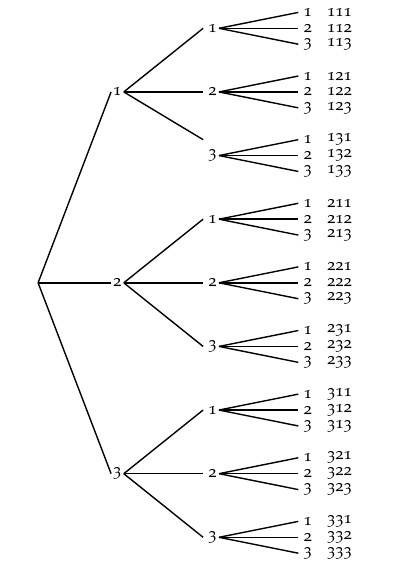
\includegraphics[scale=0.45]{images/arbol_pos.jpg}
    \end{center}
    
    %\vskip 8cm
    \vskip .2cm ¿Cómo justificamos esto? \pause Por el principio de multiplicación
    \end{frame}
    
    \begin{frame}    
        
        De los dos ejemplos anteriores se podría inferir que hay $3^4$ formas posibles de elegir en forma ordenada $4$ elementos del conjunto $1$, $2$, $3$. También, que cuando elijamos $5$ habrá $3^5$ posibilidades y así sucesivamente para enteros más grandes. 
    
        \pause 
    
        \vskip .2cm ¿Cómo justificamos esto? \pause     Por el principio de multiplicación
    
        \pause 
    
        \vskip .2cm Hemos visto en las página anteriores que hay $3^3$ formas posibles de elegir $3$ números entre $1$, $2$, $3$.
    
        \vskip .2cm Ahora,  para elegir el cuarto número hay $3$ posibilidades, por lo tanto, por el principio de multiplicación, el número de posibilidades  con cuatro elecciones es
        \begin{equation*}
            3^3 \times 3 = 3^4.
        \end{equation*}
        \end{frame}
    
    \begin{frame}    
    
        
    El razonamiento anterior  se puede extender:
    
    %\begin{proposicion}
    \vskip .3cm
    {\color{blue} Proposición}
    \vskip .2cm
        {\it  Sean  $m,n \in \mathbb N$. Hay   $n^m$ formas posibles de elegir ordenadamente $m$ elementos de un conjunto de $n$ elementos.}
    %\end{proposicion}
    \vskip .5cm \pause
    {\color{blue} Idea de la prueba.} \pause
    \vskip .2cm
    %\begin{proof}[Idea de la prueba]
        La prueba de esta proposición se basa en aplicar el principio de multiplicación $m-1$ veces, 
        \vskip .2cm
        A nivel formal,  debemos hacer inducción sobre $m$ y usar el principio de multiplicación en el paso inductivo. 
    
        \qed
    %\end{proof}
    
    \end{frame}
    

\end{document}

